\documentclass[12pt]{article}
\usepackage{amsmath}
\usepackage{amssymb}
\usepackage{graphicx}
\usepackage{ifthen,enumerate}
\usepackage{listings} \usepackage{courier} \usepackage{pdfpages}
\usepackage{../thm}
\usepackage[left=3.8cm,top=3.8cm,right=3.8cm]{geometry}
\title{Responses for CS240 Assignment 3 Question 4}
\author{Alfred Chan -- 20392255}

\begin{document}
\maketitle
\begin{enumerate}[(a)]
\item
Consider an array $(a1,a2,a3)$, which may or may not be sorted. Then decision tree is the following:\\
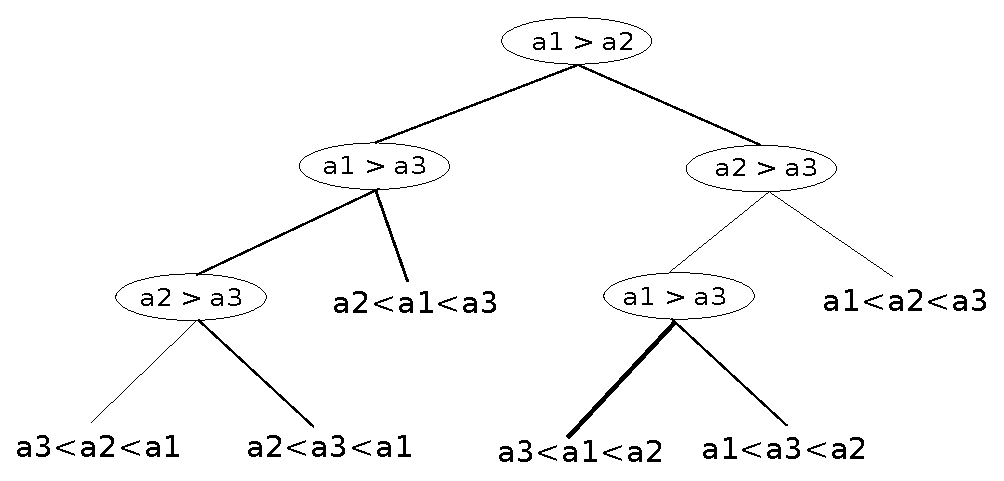
\includegraphics[scale=0.8]{decision_tree.eps}
\hfill $\blacksquare$
\item
For 3 elements, the comparison sort lower bound is
\begin{align*}
n \lg n = 3 \lg 3 \le 3
\end{align*}
But the maximum height of the above comparison tree is 3, so the array can be sorted within 3 comparisons. Therefore the worst case of insertion sort is optimal for 3 elements.
\hfill $\blacksquare$
\end{enumerate}
\end{document}

